\documentclass[output=paper]{langscibook}
\ChapterDOI{10.5281/zenodo.22796685}
\author{Alice Ray\orcid{}\affiliation{University of Orléans}}
\title[Translating \textit{Rick \& Morty}’s audiovisual novum parody]{{{Translating} }{Rick} {\&} {Morty{’s} {audiovisual} {novum} {parody:} {strategies} {and} {effects}}}
\abstract{{Since 2013}, Dan Harmon and Justin Roiland’s postmodernist TV show \emph{Rick and Morty} has staged a science-fictional world filled with dark and nonsensical humour and a tinge of nihilistic philosophy. The chapter offers an analysis of \emph{Rick \& Morty}’s invented terms that parody the genre, and their French translations in the dubbed version of the TV show. The authors use all the genre’s tools, including linguistic creativity, to ground their original world, and to generate humour. Using contrastive linguistic tools, such as semantic and morphosyntactic analysis, as well as translation studies theories and approaches, especially the notion of Nida’s dynamic equivalence, functionalist approaches to translation and previous research on translating humour, the chapter aims for a better understanding of the translation of parodic elements in a science-fictional context, especially in relation to the visual content.

The chapter offers a model for evaluating the fluency of both generic and humorous terms in the target language, using linguistic criteria, while also taking into consideration all the constraints involved in translating audiovisual material, as well as the relationship between text and image. Translation strategies may create distinct effects on the target audience as fictive terms are necessarily connected to the visual and narrative content. The analysis aims to provide a refined vision of the priorities and restrictions in play during the translation process of novum parody. Thus the chapter highlights the close relationship between text, image and translation choices. Translators prioritize one of the aspects of the invented terms (humour, parody or genre) according to the audiovisual context. The chapter also offers to validate the proposed model by analysing another audiovisual work, \emph{Futurama}, in order to confirm the hypotheses.
\keywords{science fiction, humour, audiovisual translation, dubbing, \textit{Rick \& Morty}, fictive terms, novum, dynamic equivalence, skopos theory}

}
\IfFileExists{../localcommands.tex}{
  \addbibresource{../localbibliography.bib}
  \usepackage{tabularx,multicol}
\usepackage{url}
\urlstyle{same}

 
\usepackage{langsci-optional}
\usepackage{langsci-lgr}
\usepackage{langsci-gb4e}

\usepackage{paralist}
\usepackage{enumitem}
\usepackage{cprotect}
\usepackage{fancyvrb}

\let\clipbox\relax
\usepackage[export]{adjustbox}
\usepackage{array}
\usepackage[normalem]{ulem}
\usepackage{langsci-branding}
\usepackage{langsci-bidi}
\usepackage[linguistics]{forest}

  
\makeatletter
\let\thetitle\@title
\let\theauthor\@author
\makeatother

\newcommand{\togglepaper}[1][0]{
   \bibliography{../localbibliography}
   \papernote{\scriptsize\normalfont
     \theauthor.
     \titleTemp.
     To appear in:
     E. Di Tor \& Herr Rausgeberin (ed.).
     Booktitle in localcommands.tex.
     Berlin: Language Science Press. [preliminary page numbering]
   }
   \pagenumbering{roman}
   \setcounter{chapter}{#1}
   \addtocounter{chapter}{-1}
}

\newbool{bookcompile}
\booltrue{bookcompile}
\newcommand{\bookorchapter}[2]{\ifbool{bookcompile}{#1}{#2}}

\newcommand{\qual}[1]{`#1'}
\newcommand{\bv}[1]{(\ref{#1})}

\newcommand{\ip}{ImPost}
\newcommand{\ipadv}{ImPost-adverbial}
\newcommand{\pradv}{ProxPost-adverbial}
\newcommand{\chisq}{Chi-squared}


% for rotated columns
\newcolumntype{T}[2]{%
    >{\adjustbox{angle=#1,lap=\width-(#2)}\bgroup}%
    l%
    <{\egroup}%
}
\newcommand*\rot{\multicolumn{1}{T{45}{1em}}}%


\VerbatimFootnotes


% \newcommand{\keywords}[1]{\textbf{#1}}


%  \newcommand{\textarabic}[1]{\RL{\arabicfont #1}}

  %% hyphenation points for line breaks
%% Normally, automatic hyphenation in LaTeX is very good
%% If a word is mis-hyphenated, add it to this file
%%
%% add information to TeX file before \begin{document} with:
%% %% hyphenation points for line breaks
%% Normally, automatic hyphenation in LaTeX is very good
%% If a word is mis-hyphenated, add it to this file
%%
%% add information to TeX file before \begin{document} with:
%% %% hyphenation points for line breaks
%% Normally, automatic hyphenation in LaTeX is very good
%% If a word is mis-hyphenated, add it to this file
%%
%% add information to TeX file before \begin{document} with:
%% \include{localhyphenation}
\hyphenation{
    par-a-digm
}

\hyphenation{
    par-a-digm
}

\hyphenation{
    par-a-digm
}

  \togglepaper[1]%%chapternumber
}{}

\begin{document}
\maketitle
%\shorttitlerunninghead{}%%use this for an abridged title in the page headers

\section{Introduction}

It is common to hear that humour is untranslatable or that it gets lost in translation. However, many researchers have demonstrated that this is not always the case (\citealt{Low2011}; \citealt{Hofstadter1998}; \citealt{delabastita_traductio_1997} and \citealt{delabastita_you_1997}; \citealt{Gottlieb1997}). Every language element can be adapted and adjusted according to the context. In fact, some adaptations and adjustments may be required to achieve dynamic equivalence, that is to generate the same \textit{effect} on the target audience, or at least to fulfil its function in the target culture. In fact, “translatability does not require that the TT [target texts] use the same linguistic structure, but merely that it deliver, broadly speaking, the same joke [sic]” \citep[60]{Low2011}. Besides, what is funny or not is dependent both on culture and on individuals, making the translation of humour all the more complex. Of course, language or culture-specific humour demands more creativity from the translator, as the solution may not be straightforward and may require the use of transcreation to “suit the characteristics of an intended audience” (\citealt{Díaz-MillónOlvera-Lobo2021}).

\citet{Zabalbeascoa1996} established a translation model, specifically regarding TV comedy, based on priorities and restrictions, with the priorities “as a means of expressing the intended goals for a given translation task and the restrictions are the obstacles and problems that help justify one’s choice of priorities and, ultimately, the solutions adopted in the translation” (p. 243). Of course, when translating (dubbing) TV comedy, the difficulty of transferring humour is coupled with the inherent constraints (restrictions) of the media: lip synchronization and isochrony. In our case, \textit{Rick \& Morty} being an animated TV show, the degree of tolerance for differences in lip synchronization is higher than a comedy with live actors, as the lip motion is recreated even in the source language and may not be completely accurate in any case. However, translators may still be dealing with synchronization constraints, especially isochrony: the characters – animated or not – cannot be seen talking when they are not and vice versa, or otherwise the illusion is shattered, and the audience cannot experience the show properly. Another restriction that may occur during the translation of TV comedy is the differences that may emerge “in the background knowledge of the original and prospective audiences;\footnote{\textit{Rick \& Morty} offers a perfect example in Season 6, when the authors made the character of Joseph Campbell appear: this is a reference that the target audience may not have understood.} differences in cultural and moral values, customs and traditions; differences in conventional themes and techniques of joke-telling” \citep[248]{Zabalbeascoa1996} and the relationship between the visual content and the dialogue can also be a source of challenge as it can limit creative solutions. However, all the restrictions can be overcome with creativity, by adjusting the humour to the context and the target audience, as “[w]hat matters in this case is the perception of the source text’s humour as a basis for the decision to make the translation a humorous text” (p. 247), the goal being to achieve “popularity and [create] a faithful following” (p. 245).

One of the specificities of science fiction is its use of language to stage new concepts and objects that are not real and create the cognitive estrangement of the genre as defined by Suvin: “SF is, then, a literary genre whose necessary and sufficient conditions are the presence and interaction of estrangement and cognition, and whose main formal device is an imaginative framework alternative to the author’s empirical environment” (\citealt{Suvin2016}: 20, emphasis removed; see \citealt{Spiegel2008} for a re-evaluation of the cognitive estrangement). The idea behind the concept of cognitive estrangement implies that the genre naturalises alien elements (novums) by giving them plausibility, a sense of realism. The novums, the “(novelty, innovation) validated by cognitive logic” (\citealt{Suvin2016}:~79), create a new (or partially new) paradigm that helps to rationally embroider a new world. One of the tools of sci-fi writers is fictive terms, that is, all the neologies used to name novums and create a lexicon that \textit{could possibly be} and is in fact already used as familiar linguistic artefact in the fictive world. Fictive terms often describe pseudo-scientific or pseudo-technological novums and most of them are rooted in the audience’s knowledge of the world:

\begin{quote}
Fictive neologies have a paradoxical function. They conjure up a sense of the inevitability of a new thing, or of a new discourse in which the neologism is embedded. If there is a word for it, it must already exist. And so the future must also already exist. The more convincing it is in creating an illusion of projected historical reality, the more successful the neology. Yet fictive neology also displays that it is fiction. Because the future cannot exist yet, we know that the neology is a playful, poetic conjuring device, suggesting that any imaginable future is always a poetic construction. (\citealt{csicsery-ronay_seven_2008}:~13)
\end{quote}

The translation of science fiction has been the object of previous research (\citealt{Gouanvic1997} and \citealt{Gouanvic1999}; \citealt{Wozniak2014}; \citealt{Ray2019a} and \citealt{Ray2019b}; \citealt{Campbell2021} and others) and Suvi Korpi has established the concept of “generic fluency”: “related to the quality of reception rather than textual fluency. A translation of a SF text is suggested to be regarded as generically \textit{fluent} when it preserves the voice of the genre, the fictive neologies” (\citealt{Korpi2021}: 91). Although neologies may not be the main world-building tool in some sci-fi works, when fictive terms are present in the original source text, they are of great importance as they are used to anchor the new world into pseudoscientific plausibility and credibility and “the translators play an important role in preserving the genre-typical elements as the voice of the genre” \citep[88]{Korpi2017}.

The science fiction genre has proven to be a place for humour, whether it is occasional or the global tone of the work. Science fictional humour has not been the subject of systematic research, even though some scholars wrote about specific humorous works of science fiction (\citealt{Rosinsky1982}; \citealt{Traub2018}; \citealt{Koltun2018}; \citealt{Candelaria2018}) and Dordain’s PhD dissertation (2014) attempted to define and understand science fictional humour. The same can be said about translating humorous sci-fi works.

Considering what is known about the translation of humour and the specificities of science fiction, it becomes clear that translating science fictional humour may have its own constraints, especially regarding humorous sci-fi language-related elements. \textit{Rick \& Morty} is a perfect example of a work of humorous sci-fi and uses many fictive terms as a world-building tool. The aim of the chapter is to understand how language is used to create parody in the TV show, and the way these parodic fictive terms are dubbed into French, whether they retain their generic features and their parodic nature, or if the constraints (linguistic or technical) may have changed the priorities to retain only one of the fictive terms’ features (or none). Another research topic here is if the chosen priorities consider the visual context of the term during its translation. If fictive terms are hybrids by nature, humorous fictive terms may contain oppositional features, as they must remain cognitively estranged with lexical plausibility as well as a tool for parody and humour. Taking an interdisciplinary approach, the chapter’s research uses both the conceptual tools of translation studies and of linguistics.

First, \textit{Rick \& Morty} will be introduced to define the difficulties arising from the very nature of the show, and the methodology used to conduct the research will be explained. Then, I will categorise the linguistic creativity employed in the TV show as \textit{Rick \& Morty} displays many different uses of linguistic creativity, but only one will be analyzed in the chapter, “novum parody”, that is the humorous fictive terms that parody the science fiction genre. Then, the parodic strategies of those terms will be analyzed to understand the way they were created and to linguistically explain why they can be considered as “novum parody” and “humorous”. The following sections will focus on their French translation, especially the translation strategies regarding generic fluency (see above, \citealt{Korpi2017} and \citealt{Korpi2021}) and what I will call humour fluency (i.e. the retention of the humorous features of the terms). I will also focus on the translation effects (i.e. the potential reception of the terms in the target culture) regarding the concept of priorities and the visual component of the text. In the third section, the categorizations established thanks to the linguistic creativity of \textit{Rick \& Morty} will be tested on another humorous science fiction show, \textit{Futurama}. Finally, the chapter’s analyses will provide a basis for concluding our findings and determining the treatment of the relationship between parody, genre and humour in an audiovisual work. A list of the used abbreviations in this chapter can be found at the end.

\section{Corpus and methodology}

\subsection{Rick \& Morty}

\textit{Rick \& Morty} is an animated TV show created by Justin Roiland and Dan Harmon. It first aired in 2013 and it ran for 8 seasons. The audience follows Rick, a mad scientist who tries to seek comfort and solace at the bottom of the glass and Morty, his grandson, who is as insecure and naïve as his grandfather is nihilistic \citep{Abesamis2019}. Together, they go on adventures through space and the multiverse thanks to a spaceship and a portal gun (a device that opens portals through space). The show is, I think, one of these perfect examples of postmodernist humour using satire and absurdism to highlight the grotesque nature of our societies and question our social constructs and beliefs: “\textit{Rick and Morty} is full of rich references to existential and absurdist philosophy, which are consistently used to satirise and belittle traditional social constructs such as the institutions of marriage, family, religion, and government” \citep[101]{Koltun2018}. The first sentence Genovesi writes on the show in his article is to state that “\textit{Rick \& Morty} is not an easy show to watch. It is cynical and loud, has very dark humour, and systematically deconstructs everything in which Western society used to believe” \citep[2]{Genovesi2020}. Rick is an absolute genius, aware of the presumable meaninglessness of life and of the universe. For him, nothing matters, and there is no purpose to anything:

\begin{quote}
Indeed, the very meaning of the consequences of human actions and decisions are meaningless since there are other universes in which alternative actions and decisions are taken and to where it is always possible to flee. Even if we decide to do some good, we know that in some alternative reality our counterpart is making the bad decision and causing harm instead. There is no way of avoiding the emergence of suffering and injustice in the multiverse \citep[12]{Genovesi2020}.
\end{quote}

Watching the show, the audience faces a double dichotomy: it is simultaneously “dark and hilarious; profound and stupid” \citep{Miranda2017}. We laugh with Rick at the absurdity of life itself so that we don’t cry, just like he drinks to forget he knows that nothing makes sense. The TV show was adapted into French by Xavier Hussenet, Thibault Codevelle et Soriya Leang.

To stage a postmodernist nihilistic vision of human (and extraterrestrial) life, the authors of \textit{Rick \& Morty} have chosen to parody and explore science fiction tropes. Indeed, they offer the perfect tools to highlight cultural relativism, universe meaninglessness, and the dismay of human lives by creating satire through alien environments and absurdist situations\footnote{In the episode “Anatomy Park”, Morty is shrunk to save an amusement park built inside the body of a man.} that still display cognitive estrangement, thus enhancing the relationship between the show and the audience’s reality:\footnote{Even though the situations are absurd, they are supported by novums and pseudo-scientific and pseudo-technological explanations. They may seem plausible.}

\begin{quote}
It explores, and often trivialises, traditional science fiction tropes using clever and dark humour, with the fundamental example being the perverse spin on \textit{Back to the Future’s} Doc and Marty character dynamic \citep[101]{Koltun2018}.
\end{quote}

The authors use the specificities of the genre to create humorous situations, especially with the concept of novum. Of course, some novums are quite far-fetched in the show, but as long as they are (or can be) rationally explained in the science-fictional world, they are plausible and may enter the xeno-encyclopedia.

\begin{quote}
Humour interacts in a very specific way with some science fictional features. The process gives rise to a distinctive form of humour: science fictional humour. It draws on the creative power of science fiction to offer innovative and original inventions designed to induce laughter (\citealt{Dordain2014}: 494, my translation).
\end{quote}

The TV show abounds with absurd concepts and objects that are named by the author to highlight their absurdist and humorous nature (“The Machine of Unspeakable Doom”, “the real fake doors”, “plumbus”, to name but a few of them).

\begin{quote}
From the point of view of humour, the xeno-encyclopedia allows authors to conceive creatures, concepts and places that precisely meet their needs without bothering about realism, or even verisimilitude, so that they can produce humorous scenes (\citealt{Dordain2014}: 374, my translation).
\end{quote}

All forms of humour constantly overlap during episodes, creating very dense and sometimes hard-to-follow stories. However, the substantiality of the show and the fact that it needs to follow the codes of the science fiction genre create a real challenge for translators who must also follow the technical rules of dubbing: isochrony, lip synchronization, and characters’ language specificities. The translation of audiovisual comedies, whether via subtitling or dubbing, has been previously studied in numerous articles and books (\citealt{Zabalbeascoa1996}; \citealt{Attardo2002}; \citealt{Martínez-Sierra2006}; \citealt{Bucaria2008}; \citealt{Jankowska2009}). The one element that clearly emerges from the research is the fact that humour is culturally bound and its translation may be a real challenge in that respect, especially when coupled with technical constraints and no possibility of footnotes:

\begin{quote}
The translation of cultural elements becomes even more complicated when a movie [or any audiovisual works for that matter] has to convey entertaining factors and a translator has to face various humorous phrases, wordplay, allusions, irony, or idiosyncratic metaphors. It follows that humor contains a wide array of linguistically and culturally based expressions, which make a translator’s work difficult because some elements seem to be hardly translatable \citep{Burczynska2012}.
\end{quote}

Some researchers have already offered models for understanding translation strategies regarding humour and helping translators deal with humour. \citet{Zabalbeascoa1996} offers a model of translation based on priorities (the intended goals in the translation) and restrictions (the obstacles and problems justifying the choice of priorities). All depend on the type of audiovisual work, of course, but concerning TV comedy (animated or not), the priorities are clearly to entertain, be funny, and then achieve popularity \citep[245]{Zabalbeascoa1996}. His model classifies jokes from the translator’s perspective: the international joke; the national-culture-and-institutions jokes; the national-sense-of-humour-joke; the language-dependent jokes; the visual jokes and the complex joke. Martínez-Sierra proposes to complete the model with another classification: Community-and-Institution; Community-Sense-of-Humor; Linguistic; Visual; Graphic; Paralinguistic; Sound; Non-Marked \citep{Martínez-Sierra2006}. The strategies deployed to translate the jokes will depend on both priorities and restrictions but also on the type of jokes.

\citet{Attardo2002} also offers a metric to approach humour translation using the six Knowledge Resources of the General Theory of Verbal Humour: Language, Narrative Strategy; Target; Situation; Logical Mechanism; Script Opposition. All the Resources are classified in a linear scale and “the degree of perceived difference between jokes increases linearly with the height of the Knowledge Resource in which the two jokes differ” \citep[183]{Attardo2002}.

Thus, according to the humour displayed in the source text, translators may have to find creative solutions and sometimes even completely adapt the joke to achieve the same effect of the audience (or not, according to the given priority – see \citealt{Zabalbeascoa1996}). There also remains the question of censorship and acceptability that can be linked with humour, as it is culturally bound, and each culture has its own boundaries. \citet{Bucaria2008} is interested in the ways dark humour crosses cultures in audiovisual translations (English and Italian languages) and concludes that dark humour is mostly transferred in Italian, and when omitted, it is more probably because of linguistic or technical constraints than censorship or acceptability. That may not be the case in every culture or/and for every type of humour.\footnote{In the TV show \textit{Friends,} for example, the character Monica says to Joey and Chandler “Rachel and I will kiss for one minute” and it was dubbed into French as “Rachel et moi on vous embrasse pendant une minute”, shifting the classic heterosexual male fantasy of two women kissing each other into a more “traditional” proposal of two women kissing two men.}  \textit{Rick \& Morty} offers a new perspective on the question as humour is combined with science fiction’s cognitive estrangement. The models previously proposed by researchers (especially \citealt{Attardo2002} and the use of the General Theory of Verbal Humour in relation to translation) do not consider the specificities of science fiction or science fictional neologies. A new model must be developed to understand the intricacies of the fictive terms and the translation challenges they create.

\subsection{Methodology}

To understand how \textit{Rick \& Morty}’s fictive terms are transferred into French and to analyse whether it is possible to retain both the science fictional and humorous features of the terms, all the science-fiction language-related elements were extracted from Seasons 1 to 4 in the source text as well as their dubbed French translations.\footnote{The analysis of the humorous and science fictional features of the terms also drew on my linguistic skills as a French native speaker.} According to their context, they were divided into three categories I will detail in the analysis section: fictive terms, referential parody, and novum parody. To answer the research question, the focus of the chapter will be on novum parody as they are the fictive terms with the most humorous traits. 388 terms were identified out of the 1,139 extracted. The analysis I propose in the chapter is both quantitative and qualitative.

After the extraction and categorization of the fictive terms, all the terms falling under the category “novum parody” were analyzed and categorized to answer the question: how are the terms created in the SL? Nine categories were identified and each one of them is based on objective linguistic criteria (morphosyntactic and semantic).

Then, the corresponding target terms were analyzed to clarify whether they retained both the science fictional and humorous features of the source terms following Korpi’s concept of generic fluency and the two strategies identified in her work: retentive strategy and recreative strategy. Then, I analyzed the humorous aspects of the terms in the dubbed version, and three translation strategies were identified: non-parodic, adaptative, and preservative.

Finally, to clearly identify whether novum parody terms are both cognitively estranged and humorous in the French dubbing, four translation effects were established according to the previous strategies and the visual and narrative context of the terms as “A competent translator should be able to recreate the images that the source text tends to generate in the audience” (\citealt{ElejaldeSáenz2020}: 47).  The audiovisual nature of the show implies a strong connection with the visual content, and as in any artistic work, the context of the terms is also crucial to create a particular effect on the audience. I established four different translation effects based on linguistic criteria and the broader context of the terms,\footnote{It should be interesting to compare our results with questionnaires on real spectators.}  they will be defined during our analysis section: omission, humour, cognitive estrangement, and full retention.

The categorizations that are offered here were the results of my own analysis which has been later reviewed by my colleague Mr.~Thierry Robin, professor in English Literature and Language, whom I warmly thank for his time and energy.

\section{Analysis}

\subsection{Linguistic creativity}

\textit{Rick \& Morty} displays tremendous linguistic creativity not only to consolidate the sci-fi universe, but also to make the audience laugh and to develop the characters. After the extraction of all science fiction language-related elements, three types of linguistic creativity were identified:

\begin{itemize}
\item Fictive terms: typical invented terms that can be found in many science fiction works. They describe novums as rooted in our scientific and technological knowledge. Even if the science displayed is not quite accurate (or is completely extrapolated), the concepts or objects named with fictive terms have a rational explanation in the science-fictional world. Many fictive terms are coined using pre-existing languages (Latin, Greek, English, French, etc.) and usual word-formation patterns \citep{Gindre1999}. Some others are in fact neosemes; they can already be found in dictionaries, but their meaning is derived to reflect a new reality.

\begin{itemize}
\item “portal gun”: N+N describing a new invention allowing characters to go from one place in the universe to another through a portal.
\item “insect”: neoseme describing a race of alien.
\item “Gazorpians”: N+suffix describing a race of alien with the typical suffix “-ian” used to indicate a relation between a person and a place.
\end{itemize}
\item Referential parody: references to other pop culture works.\footnote{The direct references such as quoting the title of the work, or the name of the artists were not included in this category as they were not considered as novums but only references.}  The authors pay tribute to a specific work or artist within the context of an episode.

\begin{itemize}
\item  “to Cronenberg the world up”: to turn people into hideous monsters resembling Cronenberg’s works with body horror.
\item “to go blade runner”: to rebel against humans, as in \textit{Blade Runner} \citep{Scott1982}.
\item “Snake Net”: a wordplay with “Sky Net”, the deadly artificial intelligence leading the robots in the dreadful war between robots and humans in \textit{The Terminator} \citep{Cameron1984}.
\end{itemize}
\item Novum parody: all the fictive terms of \textit{Rick \& Morty} that ground the science fictional world but clearly amplify some tropes and features of the genre to such an extent that they become parodic, or at least humorous. Novum parody terms are created through different linguistic devices, but their humorous features stem from science fiction.

\begin{itemize}
\item “a flumbus”: a new and weird object.
\item “to Glorzo something”: the infestation of the Glorzos (an alien race that acts as a parasite) on a person or a planet.
\item “mega-fruit”: the fruit of the mega-branches. Here, the use of an imprecise prefix for a wonderful new discovery transforms the novum into parody.
\end{itemize}
\end{itemize}

The focus of the analysis will be on novum parody, as they are lexical or phraseological creations that intertwine both science fiction and humour. Indeed, fictive terms do not contain any humorous traits and are mostly used to ground the sci-fi world and create plausible novums. On the contrary, referential parody is made to be funny and pay tribute to many of the classical texts of pop culture. However, if referential parody elements participate in the multi-referentiality of the show, their humorous features mostly lie in the references rather than in linguistic creativity.\footnote{However, some instance of referential parody use linguistic creativity to highlight the tribute: “Isaac Asi-hole” (S3E09); “She Clive Barkered herself” (S3 E05); “Are you seriously Sawing the Vindicators?” (S3E04). Referential parody deserves its own analysis regarding translation as the challenge lies on both cultural references and humour, not so much on cognitive estrangement. Maybe in our next adventure.}

To be clearer on what was considered as novum parody, here is the list of the criteria:

\begin{itemize}
\item Any new inventions, objects or concepts which exaggerate sci-fi tropes using linguistics (word-formation pattern especially).
\item Terms which are not parodic by themselves, but become so through repetition and accumulation:

\begin{itemize}
\item “alien hospital”; “alien towel”; “alien Internet” (S2E08).
\item “infinite sisters”; “infinite grandkids”; “infinite daughters” repeated in the entire show.
\end{itemize}
\end{itemize}

On the contrary, the category “novum parody” does not include:

\begin{itemize}
\item All the alien words that are supposed to be from an alien language (\textit{except} when they are used with English words).
\item Proper names (toponyms, anthroponyms and alienonyms).
\item Titles of other artistic works.
\item Terms containing the adjective “sci-fi” as these terms were considered as part of the show’s metadiscourse which also deserves its own analysis regarding translation.
\item All the insults.\footnote{Insults can be fertile ground for creativity, but they are not specifically designed to ground the sci-fi world, even though some of them use the genre to be even more creative and create new insults only understandable in the science fiction world.}
\end{itemize}

\subsection{Parodic strategies in the original}

\label{bkm:Ref155259883}

As the aim of the chapter is to evaluate the balance between the sci-fi aspects of the terms and their humorous nature in their French translation and according to the audiovisual nature of the text, there is a need first to categorise how the authors have created the comedic aspect of novum parody. After analysing all the 388 terms, nine categories were identified through specific linguistic criteria. Some terms can be classified in more than one category but, in order to facilitate the quantitative analysis, only the main category of humour was considered in the analysis.

\subsubsection{Linguistic parody}

Linguistic parody includes all the terms that highlight the absurdity of the novum through recognisable lexical patterns (“nano-doctor”, “holophobic”) as well as the terms that are supposed to show language evolution (“the boom-boom”). Some of the terms use non-existing roots that only sound like they belong to a technical or scientific lexicon through known affixes.

\begin{itemize}
\item “headward”: the humans see giant heads appear in the sky and some of them create a religion. “headward”, a clever use of the directional suffix "-ward”, meaning to go towards the heads.
\item “universe-destroying un-thought-out technology”: the accumulation of modifiers creates a term that could resemble a technical term, but the elements are in fact imprecise and non-technical (“un-thought-out”), parodying this kind of technical jargon in science fiction.
\item “defraculate”: there is no real definition of the term as Rick (or anyone) doesn’t explain what a “defraculator” does. The term uses affixes “de-” and “-ate” that are common in English words, especially in technical terms ("hydrogenate", "deactivate"; "denominative"; "degrade").
\end{itemize}

\subsubsection{Semantic parody}

Semantic parody includes all the terms whose parodic or humorous features are found in the semantic content. It is not as much the way the terms are morphologically created, but the meaning of the new collocation which is absurd or parodic (exaggerating science fictional tropes). All terms that stage an absurd novum are included in semantic parody as well as those that already exist but are redefined by the TV show through a new absurd meaning.

\begin{itemize}
\item “infinite daughter”: the repetition of the adjective “infinite” throughout the TV show highlights the absurd aspect of the collocation. It means that the multiverse is infinite, therefore Rick has an infinite number of his daughter.
\item “a perfectly realized, toilet-filled simulation of heaven”: the idea behind the term is quite absurd as “toilet-filled simulation” and “heaven” seem two opposite ideas.
\item “giant hidden camera”: the whole idea of a hidden camera is to be small and undetectable. The “giant” nature of this particular camera gives the object a humorous tone.
\item “sound-erasing sneakers”: shoes that erase any sound. By definition "sneakers" are quiet shoes thanks to their rubber soles, hence their name. The novum is humorous because the invention is inherently redundant, a pleonasm in itself, while being also absurd and pointless.
\end{itemize}

\subsubsection{Familiarising estrangement}

Familiarising estrangement includes the terms that transform familiar collocations or concepts by adding a sci-fi (often exaggerated) element. Concepts and objects sound quite familiar to the audience but are twisted to sound science fictional. It is often used in the description of alien or alien environment; thus, it is far-fetched to assume those human concepts and objects will be used as such in extraterrestrial societies.

\begin{itemize}
\item “Morphizer customer service”: a Morphizer is an alien machine that gives the ability to shrink or grow. In the episode in which the Morphizer appears, the character using it has some trouble with the controls. One piece of advice is to call the Morphizer customer service. Once again, customer service is a human concept and applying those concepts to alien technology is humorous.
\item “Planetary mindset”: the idea that someone who is born and lives on a planet has a particular way of thinking is humorous as it turns social theories to a much larger scale between the ones living on a planet and the intergalactic ones who fly around in space.
\item “Low-calorie petroleum flakes”: the liquid substance that is used to refine products or create gasoline, and that is highly toxic in our human world is in fact used by aliens as an ingredient in their cereals, but do not worry, they are low-calorie!
\end{itemize}

\subsubsection{Phonetic estrangement}

Phonetic estrangement includes all the terms that sound alien but are used alongside English words to give a sense of (alien) exoticism. This is also a parodic tool as the use of phonetically estranged words with English sentences amplify the science fictional trope that English will be used in the entire galaxy as the \textit{lingua franca}, which is quite absurd. The phonetically estranged terms are often created with unusual sounds for the English language, making them humorous.

\begin{itemize}
\item “give me the Blimfarx”: the audience has no clue as to the meaning of the word “blimfarx” when heard the first time as the sentence is pronounced in the background by an alien. The randomness of the sentence and the use of a very exotic phonetics makes it humorous. Later, it is understood that “blimfarx” is intergalactic money.
\item “To squanch”: a very versatile word used as a verb, a noun or even an adjective by a character named Squanchy from Planet Squanch. It can also be used to imitate existing word, such as “ensquanché\textit{”} for the French “\textit{enchanté”}. When used as a verb, “to squanch\textit{”} can refer to a sexual act, but otherwise the noun and adjective “squanchy” can in fact replace any other words (in a similar way to the term "smurf" or “schtroumpf\textit{”} created by Peyo for the eponymous French comic books) :

\begin{itemize}
\item “Rick! Squanchy party, bro!”
\item “I’m squanching in here!”
\item “Hey, squanchers! The party squanches out at my place”
\end{itemize}
\item “plumbus”: a device used for many different things. This object appears in a commercial video that explains how plumbuses are made.
\end{itemize}

\subsubsection{Undertechnicalization}

When visiting a science-fictional world with a mad scientist as the main protagonist, the audience expects to see many brilliant inventions with advanced technology, whether invented by the scientist or by intelligent beings. The authors play with this expectation by oversimplifying some of the inventions or discoveries. This can be attained using imprecise terms to describe pseudoscientific novums, the familiarization of scientific notions or objects with daily items or the use of the familiar register to describe pseudoscientific novums. In the context, it is a parodic strategy as the expectations of scientific or technical terms to describe the sci-fi word is counteracted by oversimplified terms.

\begin{itemize}
\item “Snake-makery”: to turn someone into a snake. The term uses the noun “snake” with a derivative “makery”. For an invention that is quite amazing (as far as I know, nobody knows how to turn people into snakes or into anything for that matter), the term does not reflect the complexity of the concept.
\item “Regular matter”: this is the opposite of dark matter. The adjective “regular” sounds very general and not scientific.
\item “Special grappling shoes”: it describes shoes that allow its owner to stick on any walls. The adjective “special” is used to name the invention but it is not a very technical term.
\end{itemize}

The spaceship is also referred to as “the thing” throughout the show: “fly this thing” or “to land the thing” as if it were any familiar object (which it is for Rick and Morty, but not for the audience) - in accordance with the formal framework of science fiction which "is not estrangement, but exactly its opposite, naturalization. On a formal level, sf does not estrange the familiar, but rather makes the strange familiar" (\citealt{Spiegel2008}).

\subsubsection{Accumulation}

The accumulation strategy involves the use and re-use of invented terms in a short period of time or repeatedly throughout the episodes. The accumulation strategy uses terms that are often parodic in themselves and so belong to another strategy; the fact that they are repeated numerous times adds the strategy of accumulation.

\begin{itemize}
\item “Gear wars”, “gear college”: the terms describe a world in which people are made of gears (“gear people”), so in a world with gear people, everything is made out of gear.
\item “Infinite daughter”, “infinite grandchildren”: as explained above, Rick travels through the multiverse and meets a great number of versions of himself, of Morty and any other characters. Thus, in his point of view, he has infinite daughters and grandchildren as the multiverse offers an infinite version of them.
\item “Defraculate”, “defraculator”, “fraculation”: in only a few seconds, all the terms are pronounced, which highlights the absurdity of the inventions that are not defined by the characters:

\begin{itemize}
\item Look, I’m not paying 70 smidgens for a broken defraculator.
\item That is multi-phase quantum resonator.
\item Well, does it defraculate?
\item No.
\item Then, it’s a broken defraculator.
\item Like you would even know dick about fraculation.\end{itemize}
\end{itemize}

\subsubsection{Metadiscourse}

One of the specificities of \textit{Rick \& Morty} is its use of metadiscourse. Repeatedly, characters, and Rick in particular, shows that he knows he is in a TV show.\footnote{“You ruined the Season 4 premiere” (S4E01); “break the fifth wall” (S4E06); the use of the adjective “sci-fi”, “a sci-fi word” (S2E06), “sci-fi friends” (S1E11).} However, the parodic strategy of metadiscourse in our chapter describes specifically the use of the characters as novums, as if they were objects or concepts of the science-fictional world themselves.

\begin{itemize}
\item “anti-Rick speech”: a speech that defies the very notion of “being Rick”. Just like there are anti-capitalist speeches, there are anti-Rick speeches.
\item “Rickless”: a character, Morty in particular, who doesn’t have a Rick by his side.
\item “a Summer”; “a Rick”; “Mortys”; “Ricks”: as all the characters have infinite versions of themselves through the multiverse, one version is randomized and can be used with an indefinite article or with a plural. The characters seem depersonalized as though they mean nothing in the whole universe which meets the nihilistic tone of the TV show.
\end{itemize}

\subsubsection{Wordplay}

The wordplay strategy involves the transformation of an existing idiom or term to create puns. The new idioms fit the science fictional world the audience is exploring while being familiar.

\begin{itemize}
\item “Plutanamo Bay”: it describes a prison on Pluto. The collocation is a transformation of an existing location in the United States, also known to be a detention camp: Guantanamo Bay.
\item “To hit dream bedrock”: in the episode, Rick and Morty are chased by a Freddy Krueger character \citep{Craven1984} in their dreams. At one point, they have reached the last level of dreams, and they can’t escape anymore in someone’s else dream (the whole episode is a crossover between Freddy Krueger and \textit{Inception} [\citealt{Nolan2010}]). This is a transformation of the idiom “to hit rock bottom”.
\item “Gorgon shit”: the authors replace the noun “bull” in the term “bullshit” by “gorgon” which, let’s assume, is the equivalent of an alien bull.
\end{itemize}

\subsubsection{Technobabble}

In science fiction, technobabble refers to all the pseudo-scientific discourses that characters use to explain complex scientific or technical phenomena. In fact, the speeches often have no scientific background, or they extrapolate altogether, but they sound scientific.\footnote{The best examples of technobabble in audiovisual science fiction can be found in \textit{Star Trek} (see \citealt{Wozniak2014}).} In \textit{Rick \& Morty}, the authors also use technobabble, but they use it in a humorous way to parody the genre, as it is clear for the audience that it is non-sense.

\begin{itemize}
\item “a couple cranks on the scaling knob with a four dilabyte cross fade would fix that in a jiff”.
\item “isolating a moment in time splitting your probable selves and shunting you into a near-duplicate equally probable reality, transporting you into it at the moment of parallel determination”.
\item “I put a spatially tessellated void inside a modified temporal field until a planet developed intelligent life”.
\end{itemize}

\subsection{Translating novum parody}

The translation of novum parody has been examined through two lenses: its science fictional aspect and its humour. For the former, the question is whether the terms retain the cognitive estrangement or if it is neutralized \citep[93]{Korpi2017}. I used the strategies established by Korpi with the concept of generic fluency: retentive and recreative. For the latter, the parodic features of novum parody translation, three strategies have been identified in our corpus: non-parodic, adaptation and preservation.

In the last part of this section, I will focus on the potential effect the translated novum parody terms have on the audience, if the translation meets dynamic equivalence (so the same \textit{effect}) or not. Indeed, as \textit{Rick \& Morty} is produced for an audience, there is a need to understand how the translation of novum parody can affect the audience: have the changes in novum parody terms completely changed their perception in the target language? Here the question focuses on the intersemiotic relation between the dialogue (and so novum parody) and the images, which, undoubtedly, impact the translation choices (\citealt{Torresi2008}; \citealt{KourdisKukkonen2015}). The analysis of the translation effects is, in the chapter, considered within the frame of linguistic criteria and the extralinguistic context.

\subsubsection{Translation strategies}

According to Korpi, if a translated science fiction text does not retain the neologies, the text is partially generically unfluent and so “the genre changes in the translation process” (\citealt{Korpi2017}: 89). The importance of neologies in defining the genre shall not be debated here, but I believe they are quite important when used by the author, and their translation can change the reception of the whole work, as they participate to the science fictional worldbuilding as well as the specific atmosphere of the work. The concept of “generic fluency” is relevant to understanding how the fictive terms are transferred from one language into another and if the estranged wor(l)ds are (re)constructed the same way in both languages. Moreover, the constraints of dubbing and the link with the visual content may determine the translation choices. With audiovisual work, novums can be contained in the visual context rather than in the dialogues, or be highlighted in both, which can offer a choice to the translator: when the novum can be seen, is the fictive term necessarily useful in the dialogue?

First, novum parody will be analyzed to understand if the cognitive estrangement of the terms is retained or neutralized in the dubbed version of \textit{Rick \& Morty.} The first strategy is “retentive”: “by choosing a retentive strategy, the translator has chosen to retain the novum’s cognitively estranging nature and preserved the neology as it is. Hence the genre remains, from the point of view of neologies, fluent in the translation” \citep[93]{Korpi2017}. The second strategy is “recreation” which consists of “the extrapolation or generalisation of the neology” \citep[93]{Korpi2017}. Thus, recreative strategy describes all the occurrences that eliminate, neutralize, or completely transform the science fictional aspect of the terms. The translator may have chosen to use their creativity to highlight another aspect of the term or compensate later on another term, because of the constraints they face. The first analysis will allow to determine whether the French dubbing is as cognitively estranged as the original version.

\begin{figure}
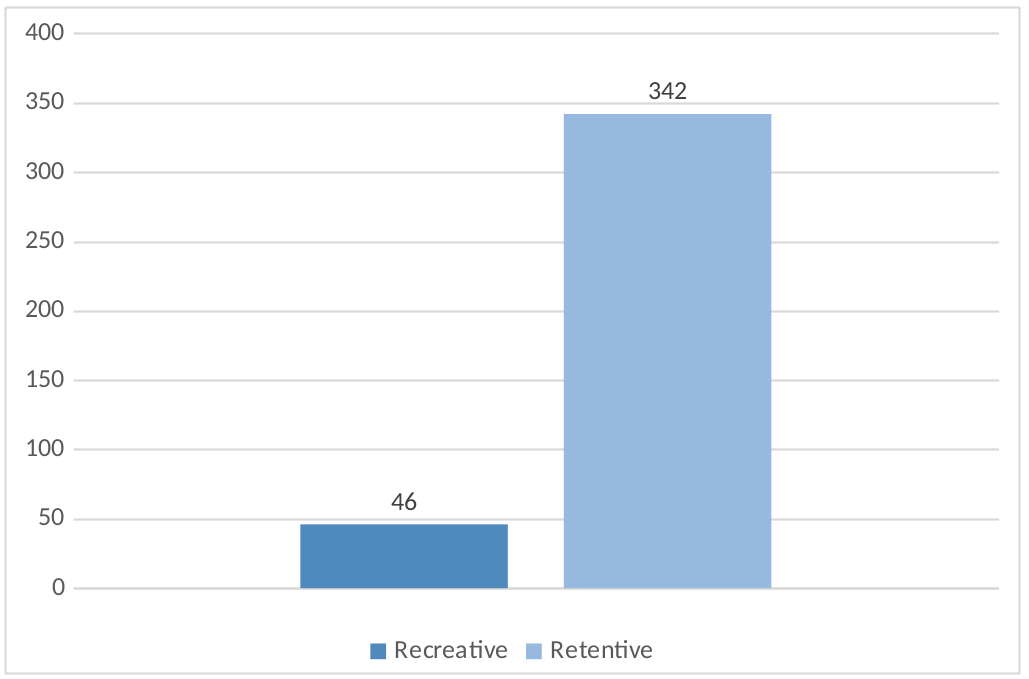
\includegraphics[width=\textwidth]{figures/RayFig1.png}
\caption{\label{fig:ray:rickmortyretentive} Generic fluency in the translation strategies of \textit{Rick \& Morty} Seasons 1 to 4's novum parody.}
\end{figure}

As seen in Figure \ref{fig:ray:rickmortyretentive}, most of the novum parody terms retain their science fictional nature as 342 (88\%) terms employ a retentive strategy while only 46 show a recreative strategy (12\%). Here are some examples of novum parody terms with a retentive strategy (\ref{ex:ray:3}, \ref{ex:ray:4}) or a recreative strategy (\ref{ex:ray:1}, \ref{ex:ray:2}):

\ea\label{ex:ray:1} SL: “shopping for a brand-new motherworld”

TL: “\textit{partir à la recherche d'un nouveau putain de monde”}

S2E10\footnote{To provide a smoother experience, each term given as an example is identified by the season and episode number in which the term is used as follows: S1E01.}
\z

\ea\label{ex:ray:2}
SL: “alien car battery”

TL: “\textit{batterie”}

S2E10
\z

\ea\label{ex:ray:3}
 SL: “headism”

TL: “\textit{tétaïsme”}

S2E05
\z

\ea\label{ex:ray:4}
SL: “The Rick-patented Anthology generator”


TL: “\textit{générateur d’anthologies breveté par Rick”}

S4E06
\z

In examples \REF{ex:ray:1} and \REF{ex:ray:2}, French dubbing neutralises the cognitive estrangement. In \REF{ex:ray:1}, the source term offers a two-layer novum: a. we can shop for a world, even figuratively; b. the idea that we can obtain a new motherworld is absurd. In the French dubbing, the estrangement is erased as the character is only talking about researching a new world for them to settle on, generalising the collocation. The same goes for example \REF{ex:ray:2} with the omission of the adjective “alien” in the French version, so there is no novum or any estrangement. Both examples are terms offering a recreative strategy. The science fictional term or collocation are transformed in the target language and lose its parodic aspects. The cognitive image projected by the terms is completely recreated in French. However, unlike science fiction literature, the cognitive image is used with a visual image that will allow some recreative translation to retain their parodic features.

On the contrary \REF{ex:ray:3} and \REF{ex:ray:4} offer a retentive strategy as “headism” and “The Rick-patented Anthology generator\textit{”} are dubbed into French with similar cognitively estranged terms. The first one is translated with “\textit{tétaïsme”}, with the same lexical pattern N+suffix and \REF{ex:ray:4} retains all the elements that give the term its science fictional features: “anthology generator”; “\textit{générateur d’anthologies}” and the fact that it is “Rick-patented”, “\textit{breveté par Rick}”. The linguistic constraints of French language require the use of a verb and a preposition “\textit{breveté par}” but the cognitive estrangement is retained.

It is interesting to note that most of the novum parody terms with a recreative strategy were categorized in “semantic parody” (13 occurrences). Many of them are translated with non-fictive terms: “childproof world” translated with “\textit{monde sûr pour les enfants}” for example, and some others were completely omitted: “turbulent power\textit{”} or “butt person”.

The visual channel can still provide the cognitive estrangement and the novum even though the fictive terms are translated through non-cognitively estranged terms or are completely omitted. The novelty is no more in the language, but it is still on the screen (in the context of the scene, not specifically at the exact moment of the lexical novum in the source language): “butt person” for example is illustrated right before the lexical novum is pronounced and so the French-speaking audience can still have access to the cognitive novum (the audience can see a person bent over with a hamster living in the person's behind). However, some of the novums are only present in the dialogue and when they are dubbed through omission or recreative strategy, they can be completely missed by the target audience. This is the case, for example with “space-skiing” translated by “\textit{en dévalant les pentes}”.

AVT is restricted by some technical constraints, especially isochrony in our case, as French actors cannot continue to speak when the characters on the screen have finished talking. As French has an expansion coefficient\footnote{“First, let’s be clear: expansion is real. It is acknowledged, even institutionalised and quantified. […] Thus, for English into French translation […], the SFT [Société française des traducteurs] predicts an expansion coefficient of 25\%” (\citealt{Durieux1990}: 55).} more important than English, some fictive terms can be a real challenge to translate in respect to time constraints. That can explain some of the recreation strategy which, as will be seen in the next section, does not necessarily mean that the cognitive estrangement is neutralized, only that it is not contained in the neology \textit{per se}. Here, the link with the visual content is the key: even though the local strategy is recreative, the reception of the term can still retain the sci-fi features. However, some terms using a recreative strategy could have been translated with a retentive strategy: “space-skiing” for example, which has been translated without any mention to the “space” nature of the sport. The answer here may be in the restrictions which change the priorities of the translators.

Once each novum parody term has been categorized according to its translation strategy in regard to generic fluency, the same must be done with its humorous features. Humour fluency has been analyzed according to three parodic translation strategies: first, the \textit{non-parodic strategy} consists of erasing all parodic features in the target language (according to the parodic strategies defined above). The term can still be humorous (especially with the visual content), but it is not parodic of the genre anymore. Then, the \textit{adaptation strategy} defines terms that are still considered as parodic, but they do not use the same humorous device as in the source language (see \ref{bkm:Ref155259883}); and finally, the \textit{preservation strategy} describes all the terms that use the same parodic strategy in both the source and the target languages (see Figure \ref{fig:ray:rickmortyfluency}).

\begin{figure}
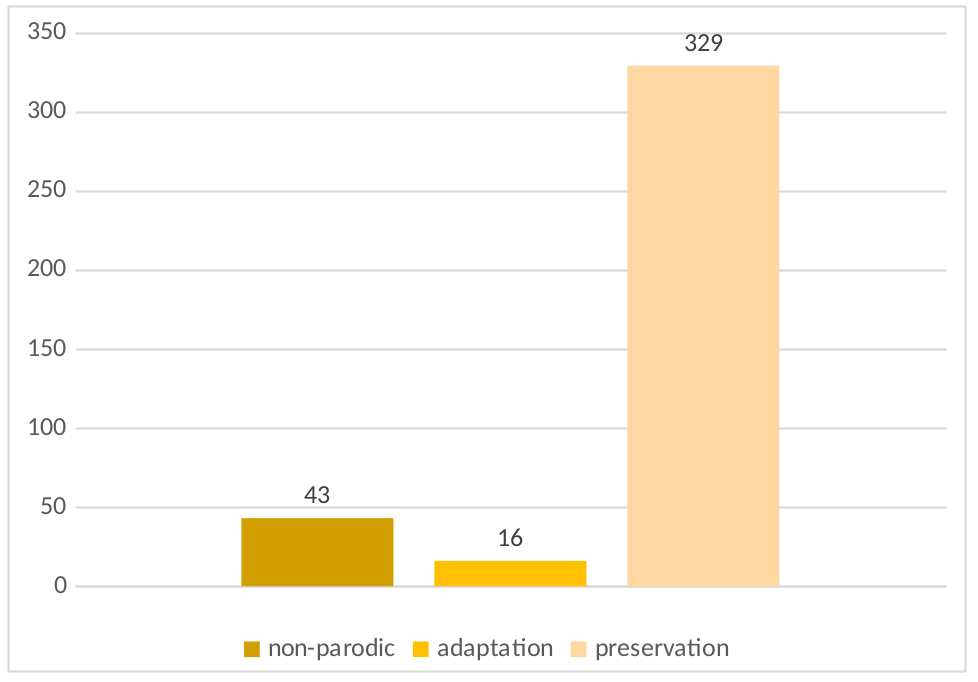
\includegraphics[width=\textwidth]{figures/RayFig2.png}
\caption{\label{fig:ray:rickmortyfluency}  Humour fluency in the translation of \textit{Rick \& Morty} Seasons 1 to 4’s novum parody.}
\end{figure}

Most novum parody has been translated with the preservation strategy and retains their humorous nature (85\%). However, 11\% has been translated through non-parodic terms and 4\% has been adapted.

\ea\label{ex:ray:5}
SL: “gear people”

TL: “\textit{créatures à mécanisme}”

S2E02
\z

\ea\label{ex:ray:6}
SL: “unprecedented Rickicidal epidemic”

TL: “\textit{vague de crime sans précédent}”

S1E10
\z


\ea\label{ex:ray:7}
SL: “six-chewable figure income”

TL: “\textit{salaire par voie orale à 6 chiffres}”

S3E01
\z

\ea\label{ex:ray:8}
SL: “worm thing”

TL: “\textit{ver de terre débile}”

S3E08
\z

Example \REF{ex:ray:5} retains the novum as the science fictional concept is preserved in the French translation. However, both the absurd collocation and the accumulation (“gear college”, “gear cream”, “gearhead”) are neutralized. The same can be observed with \REF{ex:ray:6}, “unprecedented Rickicidal epidemic\textit{”}. The audience can perceive the parodic feature of the term with the invention “Rickicidal\textit{”,} (“Rick\textit{”}+“suicidal\textit{”} as Ricks are murdering each other). In French, the novum parody is translated with “\textit{vague de crime sans précédent”,} which is an idiomatic collocation, but does not retain any of the genre or humorous features of the source term.

On the contrary, example \REF{ex:ray:7} is translated with a term that retains both generic fluency and the parodic nature of the source term. “six-chewable figure income” is dubbed with “\textit{salaire par voie orale à 6 chiffres}”. Both terms use an idiomatic collocation but transform it to fit the science fictional world. English adds the adjective “chewable\textit{”} and French dubbing adds “\textit{par voie orale”}, which is quite absurd when attached to an “income” or a “\textit{salaire}”.

In example \REF{ex:ray:8}, “worm thing” is humorous because of its undertechnicalized nature (the worm thing is an alien entity resembling a worm). It has been translated with “\textit{ver de terre débile}”, which fits the category “semantic parody” with the collocation implying that: a. a “\textit{ver de terre}” (worm) can be an alien (just like in the source term) and b. it can be stupid, and therefore the opposite can be true and a “\textit{ver de terre”} can be an intelligent being (in the human sense). Here, the linguistic parody has been adapted with a new humorous strategy, but the dubbed version retains both generic and parodic features of the fictive term.

\begin{figure}
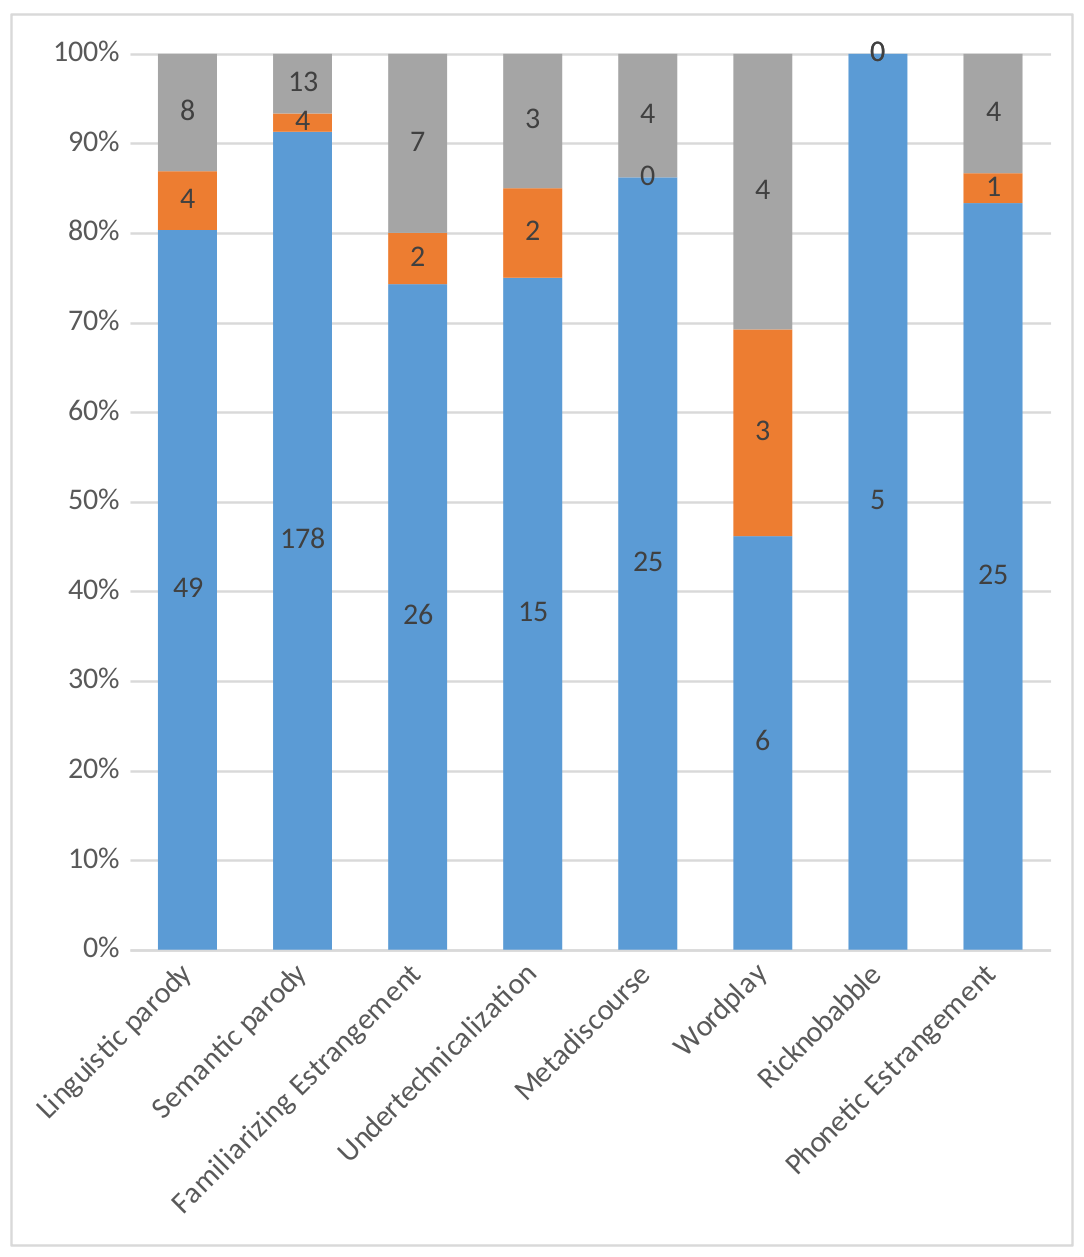
\includegraphics[width=\textwidth]{figures/RayFig4.png}
\caption{\label{fig:ray:parodicstrategies} Parodic strategies and translation strategies}
\end{figure}

It is quite clear that both science fictional and parodic aspects of novum parody are priorities for translators (see Figure \ref{fig:ray:parodicstrategiesS01}) as 329 terms are translated with a novum parody occurrence. Nevertheless, technical and linguistic constraints require the translators to adapt generic and humour fluency. The strong connection between dialogue and visual content is the key to understanding the priorities when both aspects of novum parody cannot be retained in the dubbing process. For example, “regular legged partner” is translated with “\textit{mec qui a des jambes normales}”. The translation uses a recreative strategy regarding generic fluency as the term in French is not a lexical creation anymore, it is a description that, without context, doesn’t create a new signified (it literally means “a guy with normal legs”). In English, the term uses a rather technical linguistic pattern as a parodic tool. The novum – and hence the parody – is created only through the visual content in French in which “\textit{mec qui a des jambes normales}” is visually opposed to a man who has the same legs as a baby. The translation still carries humour (not parodical anymore), but the novum relies entirely on the visual aspect of the scene.

\begin{figure}
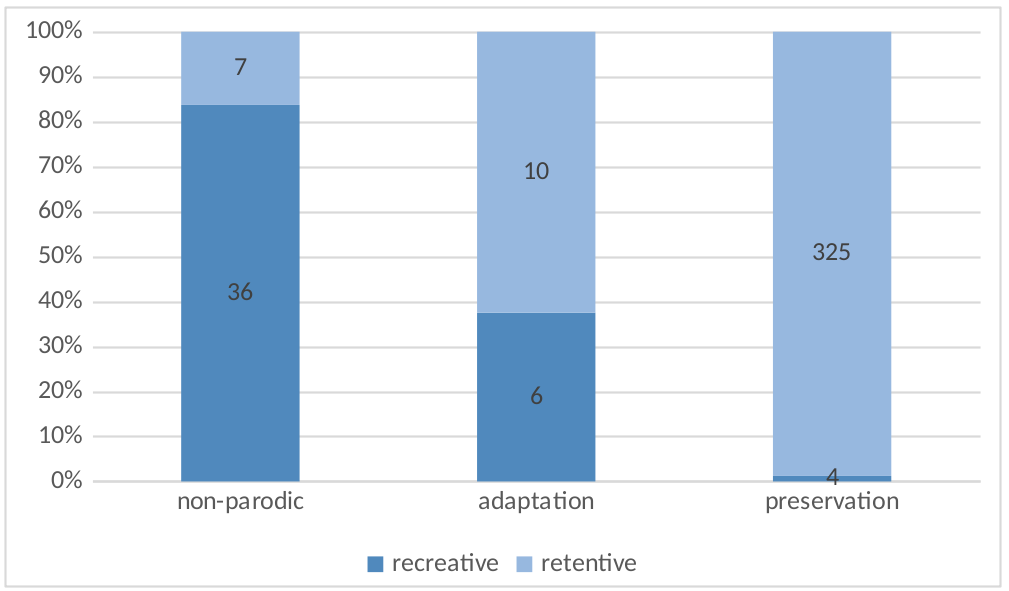
\includegraphics[width=\textwidth]{figures/RayFig3.png}
\caption{\label{fig:ray:parodicstrategiesS01}  Generic and humour fluency in the translation of \textit{Rick \& Morty} Seasons 1 to 4’s novum parody.}
\end{figure}

Looking at the percentages (Figure \ref{fig:ray:parodicstrategies}), wordplays are mostly translated with adaptation and non-parodic strategies (54\%), which can be explained by the fact that “puns [wordplay] pose special problems for translators because, unlike most kinds of verbally expressed humour, they use the specific features of a particular language” \citep[59]{Low2011}.

Furthermore, on the total of undertechnicalized and phonetically estranged novum parody, 15\% and 13\% respectively, have been translated with a non-parodic strategy. For undertechnicalization, the terms are either explained (“\textit{changer qui que ce soit en serpent}” for “snake makery”) or the sci-fi aspect of the term is neutralized (“\textit{chaussures d’escalade}” for “special grappling shoes”). In the case of phonetic estrangement, in each occurrence the element that created the estrangement is in fact completely omitted in French (“\textit{boîte special ménage}” for “Fleeseeks box” or “\textit{céréales}” for “strawberry nibbles”).

Familiarising estrangement also shows many terms translated with a non-parodic equivalent (20\%). Most of the terms are in fact translated with non-science-fictional terms. In the French version, they are still familiar terms, but they are not estranged anymore (“\textit{site de rencontre}” for “interstellar dating service”). Here, it seems that the cognitive estrangement relies, in fact, on the visual content and narrative context of the scenes.

\ea\label{ex:ray:9} SL: “egg-vite”

TL: “\textit{invitation}”

S2E10
\z

\ea\label{ex:ray:10} SL: “the bone train”

TL: “\textit{on peut y entrer qu’en passant par derrière}”

S1E03
\z

\ea\label{ex:ray:11} SL: “manipulating the fabric of shit”

TL: “\textit{sacré putain de merdier}”

S4E05
\z

In example (\ref{ex:ray:9}), the wordplay “egg-vite” is neutralized in the French dubbing and translated with “\textit{invitation}” which is a word that already exists and whose meaning is not changed within the context of the TV show. In English, the wordplay works with the visual content as the wedding invitation they receive comes in the form of an egg\footnote{The character who is getting married is a hybrid between a human being and a condor, he lives on Birdworld and is called “condorman”.} and the word “egg” has the same number of syllables as “in” and can be associated phonetically with “vite”. In French, “\textit{oeuf}” will be difficult to associate with half the word “\textit{invitation}”: “\textit{oeuvitation}” omits the last syllable of “\textit{oeuf”} and the wordplay may not be properly understood (even though the visual content is a clue) and “\textit{oeufitation}” is, in fact, not an easy term to pronounce for French speakers. The compound may not be as humorous in French, and the translator has preferred to omit it, as the visual content provides the novum (the form of the wedding invite) and therefore, the cognitive estrangement.

On the contrary, in example (\ref{ex:ray:10}), the translator has adapted the wordplay. Indeed, “the bone train” plays with the double meaning of “bone” as the part of a skeleton (they are inside a body which has been transformed into an amusement park) and the meaning “to have sexual intercourse”. In French, “\textit{en passant par derrière}” is also ambiguous as it can literally mean “to enter from behind” or “have anal sex”. Even though the translator has transformed the sentence, they have kept the sexual ambiguity of the wordplay. However, as the French expression does not refer to an object anymore “the [literal] bone train”, it is not cognitively estranged. Here, the translator decided that the priority was the wordplay, not the novum (which is visually present on the screen, even though the link between the sentence and the train is not clear in the dubbed dialogue).

The last example (\ref{ex:ray:11}) was created in the SL with undertechnicalization: “manipulating the fabric of shit”. The first part of the term “manipulating the fabric” is quite technical and sounds pseudo-scientific, but “of shit” transforms the fictive term into novum parody, playfully echoing the iconic science fiction phraseme: "the fabric of space and time". In French, the translation is still funny because of the colloquial and idiomatic language, “\textit{sacré putain de merdier}” (“holy fucking shit”), but it is not parodic anymore as there is no science fictional feature.

However, it is clear that the French dubbing mostly tries to retain the parodic nature of novum parody as the preservation strategy is the most used (85\%). Both sci-fi and parodic features of novum parody are priorities in the dubbed French version of the show. Nevertheless, some restrictions may challenge the translators who need to prioritize according to the visual and narrative context (whether the joke is more important than the cognitive estrangement or otherwise, whether the object can be seen on the screen, etc.) and the creative solutions they may come up with. That is why the local strategies which have been analyzed in this section may not be an accurate account of generic and parodic fluency. The parodic fictive terms must be analyzed with their visual and narrative contexts.

\subsubsection{Translation effects}

First and foremost, \textit{Rick \& Morty} is an entertaining TV show and as such, everything, from the fictive terms to novum parody, is produced for the audience. The reception of novum parody is essential to understanding its translation as they are not merely linguistic units but are constitutive of a whole context. Indeed, Korpi notes that

\begin{quote}{}
[n]otably the dichotomy between the retentive and recreative local strategies does not mean that using one or the other would simply guarantee the generic fluency of a text. The results indicate that many of the local strategies can be both retentive and recreative, depending on the context. \citep[94]{Korpi2017}
\end{quote}

 The translation of novum parody must also be studied according to the context, narrative and visual, in which the audience will hear them.

Using the previous analysis of generic and humour fluency, this section is dedicated to the analysis and categorization of the translation effects on the audience according to linguistic criteria. Four effects have been identified: \textit{full retention}, \textit{cognitive estrangement}, \textit{humour}, and \textit{omission}. Here the Skopos theory established in the functionalist approaches to translation (\citealt{ReissVermeer1984}; \citealt{Reiss1997}; \citealt{Vermeer2012}; \citealt{Nord2020}) will be useful, as the function of novum parody is prioritized according to the visual and narrative contexts. The translator needs to understand whether the humorous feature is more essential than the cognitive estrangement, or otherwise, when both can’t be retained because of linguistic or technical constraints.

I will use the concept of Nida’s dynamic equivalence: I considered equivalent novum parody terms that retain both generic and humorous fluency, hence creating the same \textit{effect} on the target audience (the novum parody fulfils the same function as in the source text). The functional aspect of the terms is thus taken into consideration just as much as their semantic content. As Nida noted, dynamic equivalence characterizes a translation in which “the message of the original text has been so transported into the receptor language that the response of the receptor is essentially like that of the original receptors” (\citealt{NidaTaber1969}: 200). However, because the term “equivalence” is deeply rooted in the theoretical background of Translation Studies, I prefer to use the term “full retention” to describe the terms which retain both their cognitive estrangement and their parodic features (340 occurrences), whether the translator used literal translation or chose a creative approach.  The novum or the humour can be adapted, modified according to dubbing or linguistic constraints (or even the translator’s own creativity), but the target audience is offered the same science fictional humour experience.

\ea\label{ex:ray:12} “a frog restaurant” > “\textit{un resto pour grenouilles}”
\z
\ea\label{ex:ray:13} “Alien terror attack” > “\textit{attentat terroriste alien}”
\z
\ea\label{ex:ray:14} “this magic stuff” > “\textit{ces bidules magiques}”
\z

The cognitive estrangement effect (25 occurrences) includes all the target terms that translate the science fictional novum into French without any parodic element. The term is no longer funny or absurd, but the audience can still have access to the lexical novum. Therefore, the novum parody term is generically fluent but it is not parodically fluent anymore, it becomes a plain fictive term. Translation effects take into account the visual and narrative contexts of the terms. Even though the term does not retain locally the cognitive estrangement, its use in a specific visual context can create cognitive estrangement.

\ea\label{ex:ray:15} “go into god-mode” > “\textit{avoir des pouvoirs divins}”
\z
\ea\label{ex:ray:16} “Plutoquakes” > “\textit{tremblements de Pluton}”
\z
\ea\label{ex:ray:17} “swapped our brains” > “\textit{échanger nos processeurs}”
\z
\ea\label{ex:ray:18} “special grappling shoes” > “\textit{chaussures d’escalade}” is accessible to the audience in a narrative context where the novum is explained: “grâce à ces petites merveilles de technologie, tu peux grimper sur n’importe quel type de surface, tu peux aller en haut, en bas, en dessous ou tourner à gauche. En clair, tu peux défier la gravité.” (S1E01).
\z

On the contrary, the humour effect (10 occurrences) encompasses all novum parody that does not contain any science fictional features but is still humorous. The audience has access to the comical aspect of the term, but the science fictional concept or object associated with it has been neutralized in the French dubbing. Here, however, the science fictional aspects can be conveyed through the visual channel.

\ea\label{ex:ray:19} “gold rickers” > “\textit{bande de trous du cul}”
\z
\ea\label{ex:ray:20} “a quick hand bond” > “\textit{une petite session manuelle}”
\z
\ea\label{ex:ray:21} “regular legged partner” > “\textit{mec qui a des jambes normales}”
\z
\ea\label{ex:ray:22} “interstellar dating device” > “\textit{site de rencontre}” is used by one of the characters who happens to be dating an alien. The visual context highlights the comedy aspect of the situation (the person he is dating is shown next to him on the screen and is a three-breasted blue female humanoid, so there is little doubt that she is in fact an alien).
\z

Finally, the omission effect (14 occurrences) describes all novum parody that was not translated as cognitively estranged or humorous, or not translated at all. Here the French-speaking audience loses both the science fictional and the humorous nature of the terms which become both unfluent generically and humorously.

\ea\label{ex:ray:23}  “murder log” > “\textit{carnet}”
\z
\ea\label{ex:ray:24}  “working-stiff Ricks” > “\textit{employés}”
\z
\ea\label{ex:ray:25}  “peeling skrabquams and slipping nib nibs” > “\textit{bosser comme un esclave}”
\z

\subsubsection{Translation strategies and effects}

\begin{figure}
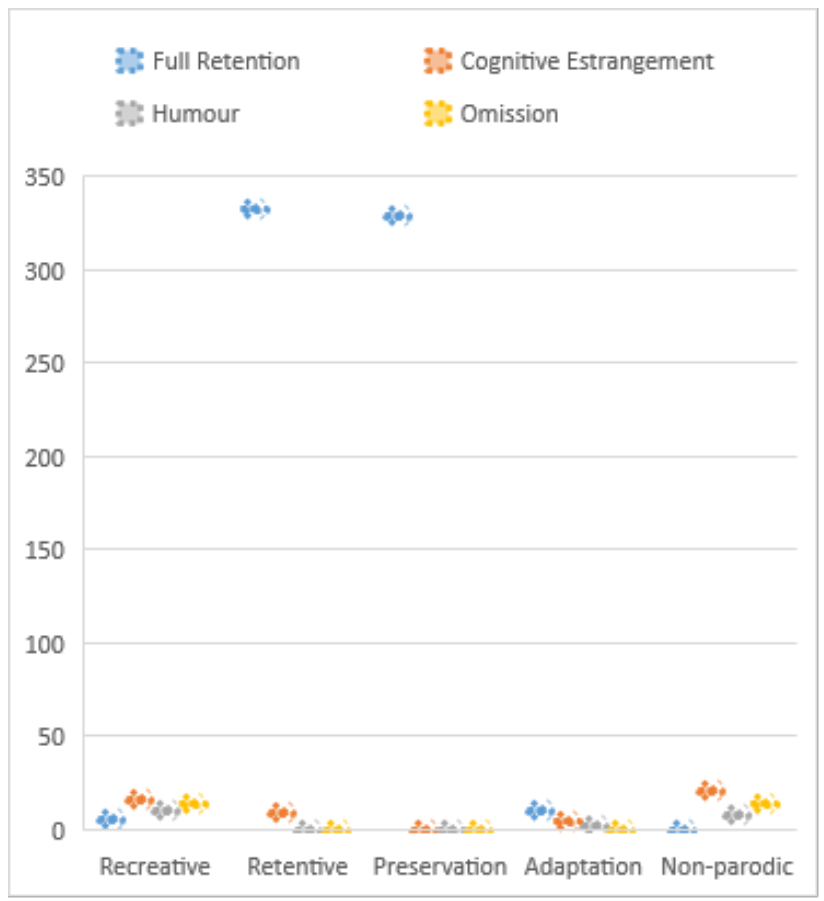
\includegraphics[width=\textwidth]{figures/RayFig5.png}
\caption{\label{fig:ray:translationeffectsandstrategies} Translation effects and strategies in \textit{Rick \& Morty}}
\end{figure}

By contrasting both translation strategies with translation effects, some interesting results have emerged (see Figure \ref{fig:ray:translationeffectsandstrategies}. For example, a substantial proportion of non-parodic terms (43) in the target language also show a recreative strategy concerning generic fluency (except for seven occurrences) and if 14 show an omission effect, most (21) fall under the cognitive estrangement effect.

Concerning the omission effect: the dubbing constraints didn’t enable the translator to transfer the lexical novum into French, but the context did not make humour a priority and so novum parody did not transform into a simple joke or a pun either. The priority appears to be in the explanation and expansion rather than estrangement or parody which can be balanced by the visual content, hence the omission of both features.

However, the cognitive estrangement effect can be created even though the translated term uses a recreative strategy. The visual component of \textit{Rick \& Morty} allows the translator to omit the linguistic novum, as its visual manifestation is on the screen or there is a narrative continuity. Thus, the translator gains time to expand another aspect of the dialogue (see example [\ref{ex:ray:18}], the “special grappling shoes”).

The same thing goes with the humour effect: even though some parodic fictive terms are not parodic anymore in the TL, the visual content and the context in which the characters are evolving can still be humorous, but the humour is only conveyed by the situation in which the words are uttered and not by the words themselves (connotation, ambiguity, etc.), see the “interstellar dating service” example.

The results show that if full retention often means retentive and preservation strategies, recreative and adaptation strategies can also lead to full retention, with the context in which the term appears or with an adaptation of the parody strategy to fit linguistic constraints:

\ea\label{ex:ray:26} “money bugs” > “\textit{la compta}”
\z
\ea\label{ex:ray:27} “gearsticles” > “\textit{avoir des testicules à la place de la bouche}”
\z

 This shows that the priorities of the translators are both the science fictional nature of the terms as well as their parodic features. However, when the constraints of AVT or the linguistic constraints from English into French are too heavy and do not allow translators to keep both features, they prioritize according to the context, visual and narrative. When humour is mostly conveyed by the term, they keep it, but when the context is funnier and the parody is only the cherry on top, they prioritize the science fictional aspect of the term. Of course, given the nature of novum parody itself, when the term is not cognitively estranged, the parody is either transformed into another form of humour, or completely neutralized. In most cases, both features are retained (87\% of full retention effect), even though one of the aspects may only be present in the visual and narrative contexts, and not in the lexical creations themselves.

\subsection{Testing the typology: \textit{Futurama}}

\textit{Futurama} is an animated TV show created by Matt Groening. It has run for eight seasons from 1999 to today, and has been produced by Fox, Comedy Central and Hulu. As \textit{Futurama} is also one example of humorous sci-fi, it seemed like a perfect choice to test the model. In brief, \textit{Futurama} tells the adventures of the Planet Express’ crew, an interplanetary delivery company in the 31st century, and especially Fry (a human cryogenized from the twentieth century), Leela (a mutant) and Bender (a robot). Although the show isn’t as nihilistic as \textit{Rick \& Morty}, it does parody the genre by exaggerating some sci-fi tropes and creating absurd situations. {The series has had several translators and Season 7 was adapted by Cécile Carpentier, Xavier Hussenet, Didier Duclos, Anne Bararuzunza, Flora Seeger, Hélène Castets, Blandine Gaydon, Émilie Barbier, Ludovic Manchette, Aurore Lafage, Thibault Longuet, Audrey Bernière, Cécile Favre et Christian Niemiec.}

To test the typology established previously, I extracted all the sci-fi language-related elements from Season 7,\footnote{Sometimes considered as Season 10 as some of the seasons were divided in two parts.} aired from  {June 2012} to  {June 2013}. I chose this season as it is the exact same year \textit{Rick \& Morty}’s Season 1 was released. Then, I extracted the same elements from the dubbed French version of the show and used the previous methodology.

105 novum parody terms were identified\footnote{Fictive terms and referential parody are also present in \textit{Futurama:} “matter compressor” (S7E01) or “deflector shield” (S7E03) which is a reference to the TV show \textit{Star Trek}.} (“padded dashboard display”; “disem”; “delay the tentacles”, for example). In terms of parodic strategies, I identified six of the previously defined categories (see Figure \ref{fig:ray:futuramaparodic}).\footnote{The category “accumulation” was found, but just like for the analysis on \textit{Rick \& Morty}’s novum parody terms, this parodic strategy is used in addition to another, and I didn’t take it much into account for the test.} However, I haven’t found any examples of “phonetic estrangement” or “metadiscourse”. For the latter, it can be explained by the differences between both shows. \textit{Rick \& Morty} uses dark humour to enhance the nihilistic discourse, and the characters (at least, Rick) are aware that they are in a TV show. In \textit{Futurama}, the characters just live their lives without any knowledge of their fictional status, and the humour is light and parodic, but not nihilistic. It resembles more a science fictional workplace sitcom in many ways.

\begin{figure}
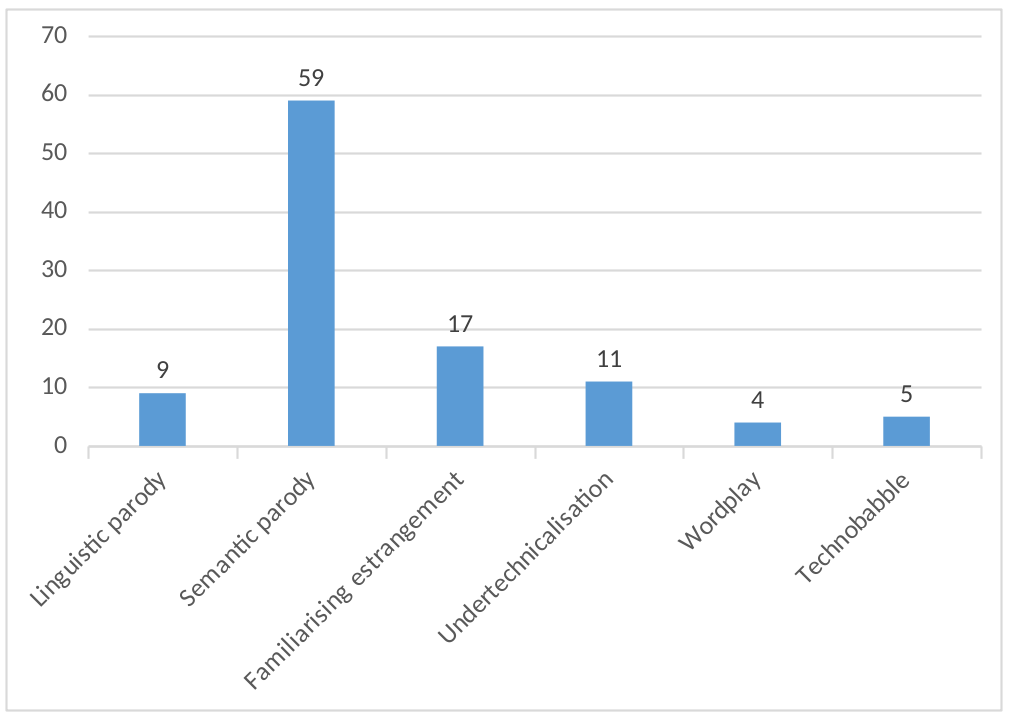
\includegraphics[width=\textwidth]{figures/RayFig6.png}
\caption{\label{fig:ray:futuramaparodic} Parodic strategies in \textit{Futurama}’s Season 7.}
\end{figure}

As can be seen in Figure \ref{fig:ray:futurameretentive}, most of the terms were translated through a retentive strategy (75\%) and most of their humorous features were preserved (73\%).

\begin{figure}
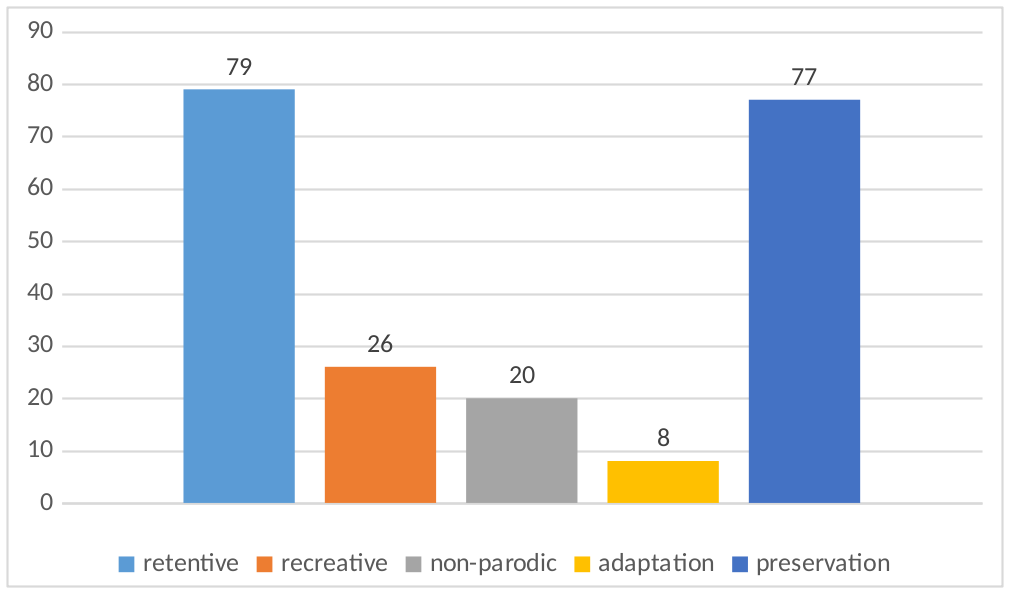
\includegraphics[width=\textwidth]{figures/RayFig7.png}
\caption{\label{fig:ray:futurameretentive}  Generic and humour fluency in the translation of \textit{Futurama's} Season 7}
\end{figure}

Here are two examples of novum parody terms to highlight the notion of priorities and how the relationship between text and image needs to be taken into account to understand translators’ choices:


\ea\label{ex:ray:28} SL: “Execubots”

TL: “\textit{Robonnets}”

E07
\z

\ea \label{ex:ray:29} SL: “Sewer Mail”

TL: “\textit{C’est le facteur}”

E09
\z

In (\ref{ex:ray:28}), the term is created through linguistic parody by merging “executives” and “robots” (as they are executive robots) and its science fictional aspect is retained in the French dubbing as “\textit{robonnets}” is also considered as a lexical novum (“\textit{robot}” + “\textit{gros bonnet”}). Here the linguistic parody is preserved in French (even amplified with the use of the familiar term “\textit{gros bonnet}” as a compound’s component).

On the contrary, in (\ref{ex:ray:29}), the novum “Sewer Mail” which implies that there is a whole organized community living in the sewers, is not dubbed as a novum in French. “\textit{c’est le facteur}” is very generic and not specifically science fictional. The familiarizing estrangement of the term is completely omitted, and the term is not linguistically humorous anymore. However, the visual content of the scene highlights the familiarising estrangement and makes “\textit{c’est le facteur}” in French humorous even though the term is not linguistically funny. Indeed, the "facteur" is shown on the screen and is obviously a mutant, creating a sense of incongruity between what is expected and what is perceived.

The translators tried to retain both the science fictional and humorous aspects of the terms. However, the visual content must also be taken into account as it can change the perception of the translated terms. One non-parodic term can still be humorous as the linguistic and temporal constraints may be counterbalanced through the visual content. Following the methodology, each novum parody term has been analyzed through the lens of the previously defined translation effects (see Figure \ref{fig:ray:translationeffectsfuturama}). Just as in \textit{Rick \& Morty}, the translators had both generic and humour fluency as priorities when dubbing \textit{Futurama}’s episodes. However, the change in tone between both TV shows produces some differences: the science fictional features of the terms were sometimes omitted to better preserve the humorous features (“foos” translated with “\textit{petits joueurs}”).

In \textit{Rick \& Morty}, most of the terms which were created through recreative or/and non-parodic strategies create a cognitive estrangement effect (when not omitted) (see Figure \ref{fig:ray:translationeffectsandstrategies}). In \textit{Futurama}, Figure \ref{fig:ray:translationeffectsfuturama} indicates that, when not omitted, the novum parody terms created through recreative and/or non-parodic strategies still create a humour (6 occurrences) or a full retention (3 occurrences) effect. Therefore, humour seems to be prioritized in \textit{Futurama} and can sometimes rely more on the visual content than on the linguistic creations.

\begin{figure}
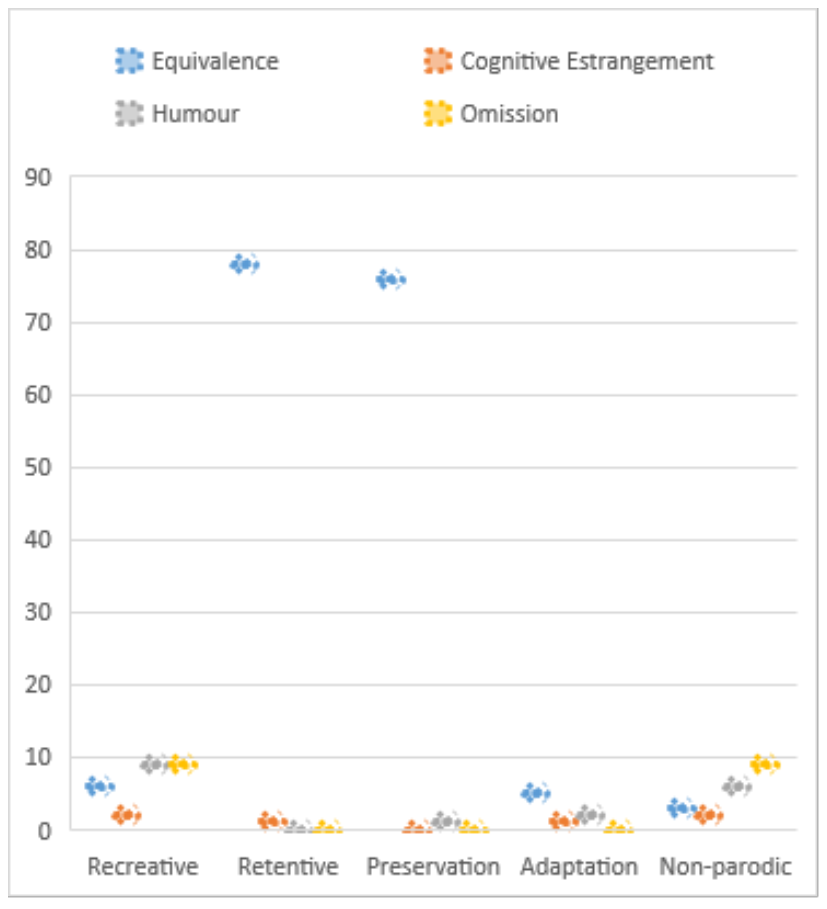
\includegraphics[width=\textwidth]{figures/RayFig8.png}
\caption{\label{fig:ray:translationeffectsfuturama}  Translation effects and strategies in \textit{Futurama’s} Season~7.}
\end{figure}

\section{Conclusion}

This chapter deals with several notions such as generic fluency and humour fluency in an animated audiovisual work. The research question focused on the treatment of the different aspects of the science fictional terms that clearly use generic parody to create humour. The audiovisual, linguistic and cultural constraints may prevent translators from offering humorous fictive terms in the target language according to the context. First, different categories of novum parody have been established to understand how the invented terms may convey generic parody in the source text; all the specificities of the language of science fiction are used by the authors to generate both humour and parody. This classification is useful for contrasting the source and target texts, and the analysis has revealed that novum parody is considered as such by the translators and that both genre and parodic features are prioritized as much as possible. Nevertheless, when AVT or linguistic constraints prevent any creative solution retaining both generic and humour fluency, the visual and narrative contexts are used to prioritize either the cognitive estrangement or the humorous aspect of the term, depending on the context or the tone.

The model suggested in the chapter is not flawless, and as any model on humour translation, subjectivity cannot be entirely dismissed. However, the model uses objective linguistic criteria to better understand the way novum parody is handled in AVT. The test on \textit{Futurama} demonstrates its relevance. \textit{Rick \& Morty} is a great object of study to further explore, especially in regard to the translation of metadiscourse and cultural references. Further research will be attempted about science fictional humour translation, particularly in audiovisual media such as TV shows or video games, to test and refine the model, so that we can get schwifty in every possible fictive world and in all languages.

\section*{Acknowledgements}

This chapter is dedicated to my Mamie who didn’t watch \textit{Rick \& Morty} or read science fiction, but she loved to laugh, and I miss laughing with her.

\section*{Abbreviations}

\begin{tabularx}{\textwidth}{lX}
sci-fi & science fiction\\
TL & target language\\
SL & source language\\
AVT & audiovisual translation\\
\end{tabularx}
\sloppy\printbibliography[heading=subbibliography,notkeyword=this]
\end{document}
